\documentclass[aspectratio=169,10pt]{beamer}

% --------------------------------------------------------------------------
% Support de soutenance — Projet 12
% Durée cible : 8 à 10 minutes (15 diapositives)
% Compilation : tectonic -X compile soutenance.tex
% --------------------------------------------------------------------------

\usepackage[T1]{fontenc}
\usepackage[utf8]{inputenc}
\usepackage[french]{babel}
\usepackage{lmodern}
\usepackage{booktabs}
\usepackage{graphicx}
\usepackage{amsmath}
\usepackage{xcolor}

\usetheme{Madrid}
\setbeamertemplate{navigation symbols}{}
\setbeamertemplate{caption}[numbered]
\setbeamertemplate{blocks}[rounded][shadow=false]

\definecolor{vert}{RGB}{0,102,92}
\definecolor{vertfonce}{RGB}{0,66,60}
\definecolor{vertclair}{RGB}{226,241,237}
\definecolor{orange}{RGB}{224,148,0}
\definecolor{gris}{RGB}{90,90,90}

\setbeamercolor{structure}{fg=vert}
\setbeamercolor{palette primary}{bg=vert,fg=white}
\setbeamercolor{palette secondary}{bg=vertfonce,fg=white}
\setbeamercolor{palette tertiary}{bg=vertfonce,fg=white}
\setbeamercolor{title}{fg=white}
\setbeamercolor{subtitle}{fg=white}
\setbeamercolor{frametitle}{bg=vert,fg=white}
\setbeamercolor{block title}{bg=vertclair,fg=vertfonce}
\setbeamercolor{block body}{bg=vertclair!45,fg=black}
\setbeamercolor{itemize item}{fg=vert}
\setbeamercolor{itemize subitem}{fg=vert}
\setbeamertemplate{itemize item}{\small$\blacktriangleright$}
\setbeamertemplate{itemize subitem}{--}

\setbeamertemplate{footline}{%
  \leavevmode\hbox{%
    \begin{beamercolorbox}[wd=.33\paperwidth,ht=2.4ex,dp=1.2ex,center]{author in head/foot}%
      \usebeamerfont{author in head/foot}\insertshortauthor
    \end{beamercolorbox}%
    \begin{beamercolorbox}[wd=.34\paperwidth,ht=2.4ex,dp=1.2ex,center]{title in head/foot}%
      \usebeamerfont{title in head/foot}\insertshorttitle
    \end{beamercolorbox}%
    \begin{beamercolorbox}[wd=.33\paperwidth,ht=2.4ex,dp=1.2ex,center]{date in head/foot}%
      \usebeamerfont{date in head/foot}\insertframenumber\,/\,\inserttotalframenumber
    \end{beamercolorbox}}%
  \vskip0pt%
}

\newcommand{\src}[1]{\vspace{0.1em}{\scriptsize\color{gris}#1}}
\newcommand{\MUSD}{\,\text{M USD}}

\title[Exportations agroalimentaires marocaines]{Prévoir les exportations de fruits du Maroc par marché}
\subtitle{Chapitre 08 du Système harmonisé, 2010--2024}
\author[Nom 1 \& Nom 2]{Nom 1 \and Nom 2}
\institute[Établissement]{Établissement \\ Data Science appliquée au commerce international}
\date{Année universitaire 2026--2027}

\begin{document}

% ---------------------------------------------------------------- 1
\begin{frame}[plain]
  \titlepage
  \vspace{-0.6em}
  \begin{center}
    {\scriptsize\color{gris}Données : UN Comtrade, API publique \emph{preview}, extraction du 31 octobre 2026.}
  \end{center}
\end{frame}

% ---------------------------------------------------------------- 2
\begin{frame}{La question, et la réponse en une diapositive}
  \begin{block}{Question de recherche}
    Peut-on prévoir la valeur exportée d'un couple \textbf{(marché, produit)}
    à un an, et les modèles d'apprentissage automatique battent-ils une simple
    \textbf{reconduction de l'année précédente} ?
  \end{block}

  \vspace{0.3em}
  \begin{columns}[T,onlytextwidth]
    \begin{column}{0.48\textwidth}
      \textbf{Ce que nous trouvons}
      \begin{itemize}
        \item Les exportations vers 6 marchés ont été \textbf{multipliées par 4,9}
              entre 2010 et 2024.
        \item La croissance est surtout \textbf{en valeur} (prix), pas en volume.
        \item La concentration reste \textbf{élevée} : 3 couples = 49,2 \% de la valeur.
      \end{itemize}
    \end{column}
    \begin{column}{0.48\textwidth}
      \textbf{Le résultat méthodologique}
      \begin{itemize}
        \item La persistance est un \textbf{benchmark très difficile à battre}.
        \item La forêt aléatoire gagne 2,9 \% sur le test\ldots
        \item \ldots mais \textbf{perd en validation glissante} : le gain n'est
              pas robuste.
        \item Conclusion : \textbf{aucun modèle ne bat la persistance de
              façon fiable}.
      \end{itemize}
    \end{column}
  \end{columns}

  \vfill
  \begin{center}
    \small\color{vertfonce}\textbf{Un résultat négatif documenté vaut mieux qu'un gain artificiel.}
  \end{center}
\end{frame}

% ---------------------------------------------------------------- 3
\begin{frame}{Données : une source officielle, un panel construit}
  \begin{columns}[T,onlytextwidth]
    \begin{column}{0.52\textwidth}
      \textbf{UN Comtrade, API publique \emph{preview}}
      \begin{itemize}
        \item Déclarant : \textbf{Maroc} (504), flux exportations.
        \item Période : \textbf{2010--2024}, 15 années.
        \item Produits : chapitre 08, \textbf{HS4 0801--0814}.
        \item Marchés : France, Espagne, Allemagne, Pays-Bas,
              Royaume-Uni, Italie.
        \item Référence : agrégats \textbf{monde} HS2 et HS4.
      \end{itemize}
      \vspace{0.2em}
      \begin{block}{Traçabilité}
        \small 45 requêtes (15 ans $\times$ 3), \textbf{0 échec}, 1\,058 lignes
        brutes, journal des requêtes livré.
      \end{block}
    \end{column}
    \begin{column}{0.44\textwidth}
      \textbf{Du brut au panel}
      \footnotesize
      \setlength{\tabcolsep}{4pt}
      \begin{tabular}{lr}
        \toprule
        Panel (6 $\times$ 14 $\times$ 15) & 1\,260 \\
        Cellules observées & 834 (66,2 \%) \\
        Zéros imputés & 426 \\
        Produits retenus ($\geq$ 50 \%) & 9 / 14 \\
        \textbf{Observations modélisables} & \textbf{648} \\
        \bottomrule
      \end{tabular}
      \vspace{0.5em}

      \footnotesize\textbf{Pourquoi 6 marchés ?} La fiche impose la France et
      l'Espagne ; les 4 autres portent l'échantillon de $\sim$200 à
      \textbf{648} observations. Le couple FR--ES reste analysé à part.
    \end{column}
  \end{columns}
\end{frame}

% ---------------------------------------------------------------- 4
\begin{frame}{Une croissance qui ne se dément pas}
  \begin{center}
    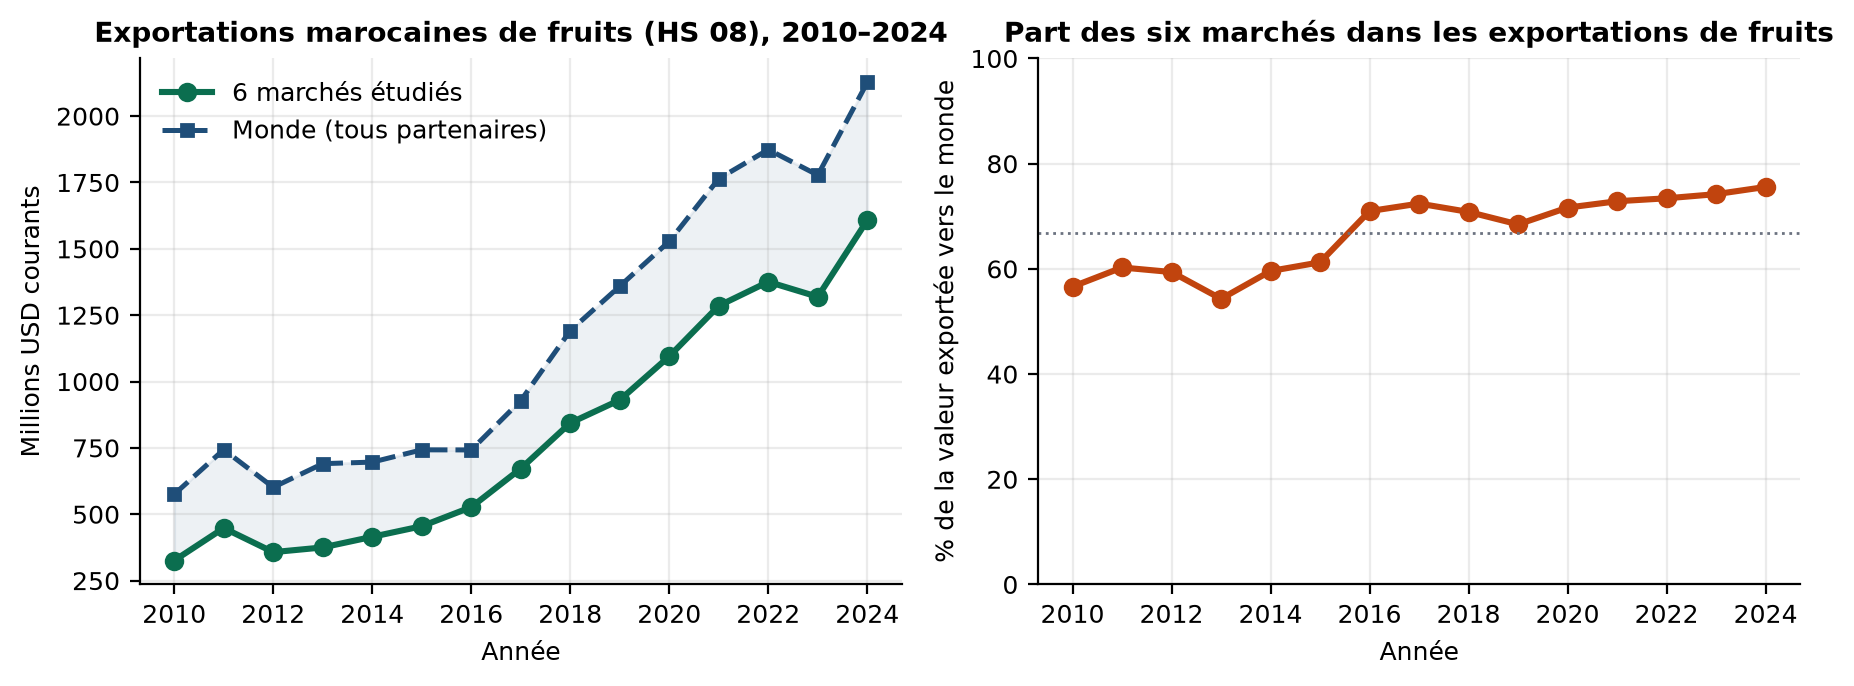
\includegraphics[width=0.90\textwidth]{../figures/fig01_dynamique_agregee.png}
  \end{center}
  \vspace{-0.5em}
  \begin{columns}[T,onlytextwidth]
    \begin{column}{0.32\textwidth}
      \centering\textbf{325,6} \MUSD en 2010\\
      \scriptsize soit 56,6 \% du total
    \end{column}
    \begin{column}{0.32\textwidth}
      \centering\textbf{1\,607,6} \MUSD en 2024\\
      \scriptsize \textbf{$\times$4,9}, TCAM 12,1 \%
    \end{column}
    \begin{column}{0.32\textwidth}
      \centering\textbf{75,6 \%} du total mondial\\
      \scriptsize moyenne 2010--2024 : 66,8 \%
    \end{column}
  \end{columns}
  \src{Source : UN Comtrade, calculs des auteurs. Montants nominaux en USD courants.}
\end{frame}

% ---------------------------------------------------------------- 5
\begin{frame}{Ce qui tire la croissance : les produits}
  \begin{center}
    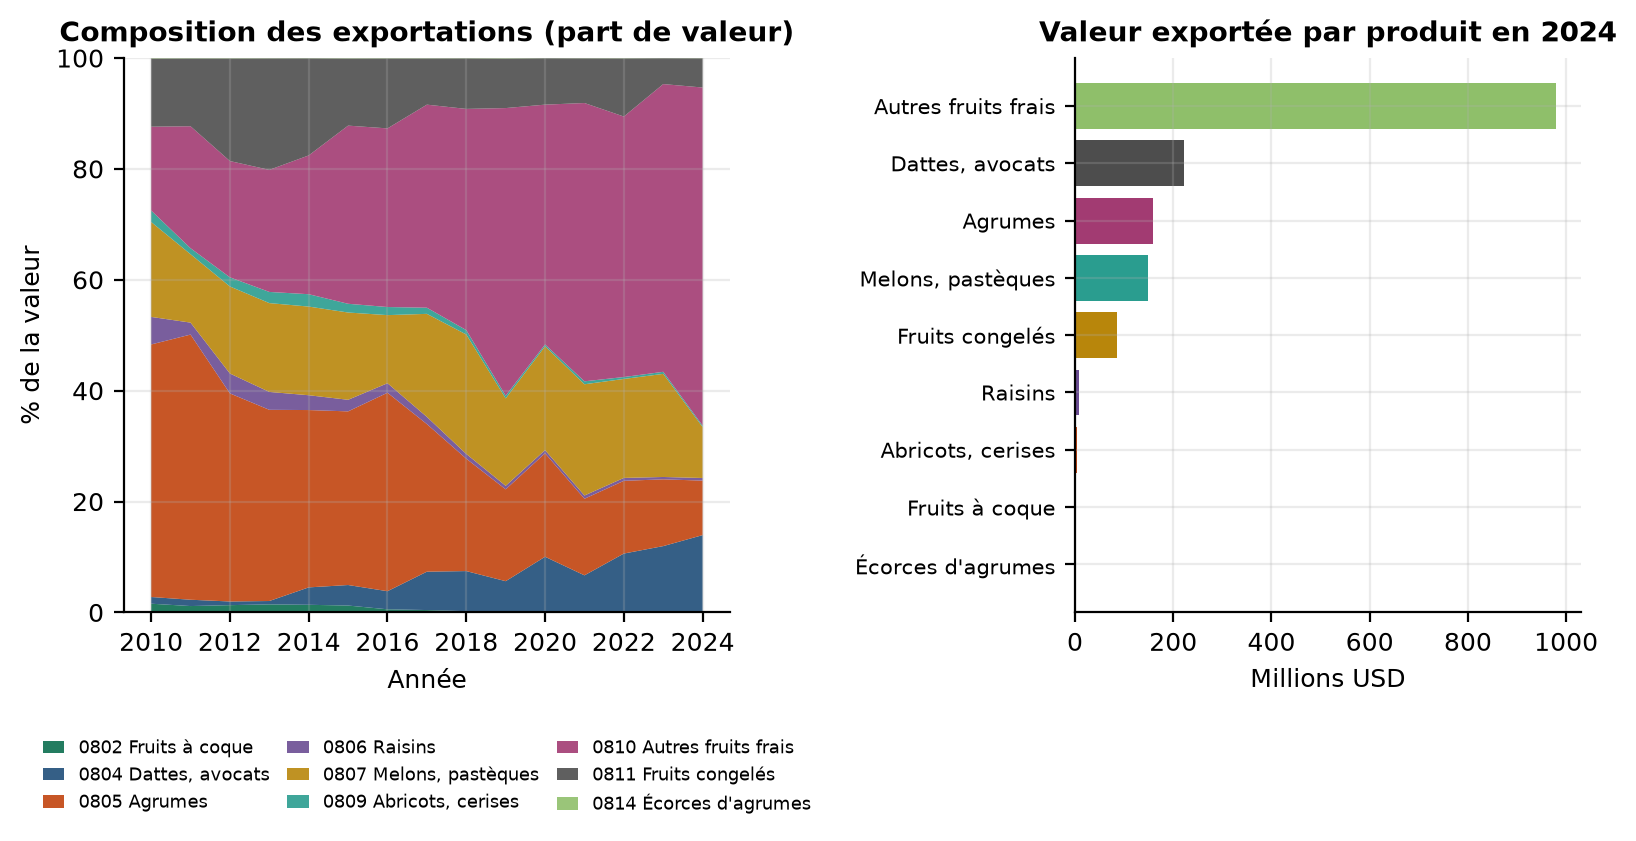
\includegraphics[width=0.74\textwidth]{../figures/fig02_structure_produits.png}
  \end{center}
  \vspace{-0.4em}
  \begin{columns}[T,onlytextwidth]
    \begin{column}{0.31\textwidth}
      \centering\textbf{61,0 \%}\\
      \scriptsize produit 0810 (autres fruits frais)
    \end{column}
    \begin{column}{0.31\textwidth}
      \centering\textbf{13,9 \%}\\
      \scriptsize produit 0804 (dattes, avocats)
    \end{column}
    \begin{column}{0.31\textwidth}
      \centering\textbf{9,8 \%}\\
      \scriptsize produit 0805 (agrumes)
    \end{column}
  \end{columns}
  \src{Parts dans la valeur exportée vers les six marchés en 2024. Le produit 0810 pèse à lui seul près des deux tiers.}
\end{frame}

% ---------------------------------------------------------------- 6
\begin{frame}{Les marchés : trois moteurs, un décrochage}
  \begin{columns}[T,onlytextwidth]
    \begin{column}{0.60\textwidth}
      \footnotesize
      \begin{tabular}{lrrr}
        \toprule
        Marché & 2024 (M USD) & TCAM 2010--2024 & Part 2024 \\
        \midrule
        Espagne & 415,6 & 19,3 \% & 25,9 \% \\
        Royaume-Uni & 390,9 & 17,7 \% & 24,3 \% \\
        Pays-Bas & 322,6 & 9,9 \% & 20,1 \% \\
        France & 313,5 & 5,8 \% & 19,5 \% \\
        Allemagne & 149,0 & 17,1 \% & 9,3 \% \\
        Italie & 15,9 & 7,9 \% & 1,0 \% \\
        \midrule
        \textbf{Total} & \textbf{1\,607,6} & \textbf{12,1 \%} & \textbf{100 \%} \\
        \bottomrule
      \end{tabular}
      \src{Valeurs en M USD courants ; TCAM = taux de croissance annuel moyen.}
    \end{column}
    \begin{column}{0.38\textwidth}
      \begin{itemize}
        \item \textbf{L'Espagne} devient le premier marché, portée par les
              fruits frais et les agrumes.
        \item \textbf{Le Royaume-Uni} double sur la période : +17,7 \% par an.
        \item \textbf{La France}, historiquement première, ne progresse que de
              5,8 \% par an et perd des parts.
        \item \textbf{Les Pays-Bas} jouent un rôle de \textbf{hub de
              réexportation} (Rotterdam).
      \end{itemize}
    \end{column}
  \end{columns}
\end{frame}

% ---------------------------------------------------------------- 7
\begin{frame}{Agrumes : la valeur monte, le volume stagne}
  \begin{center}
    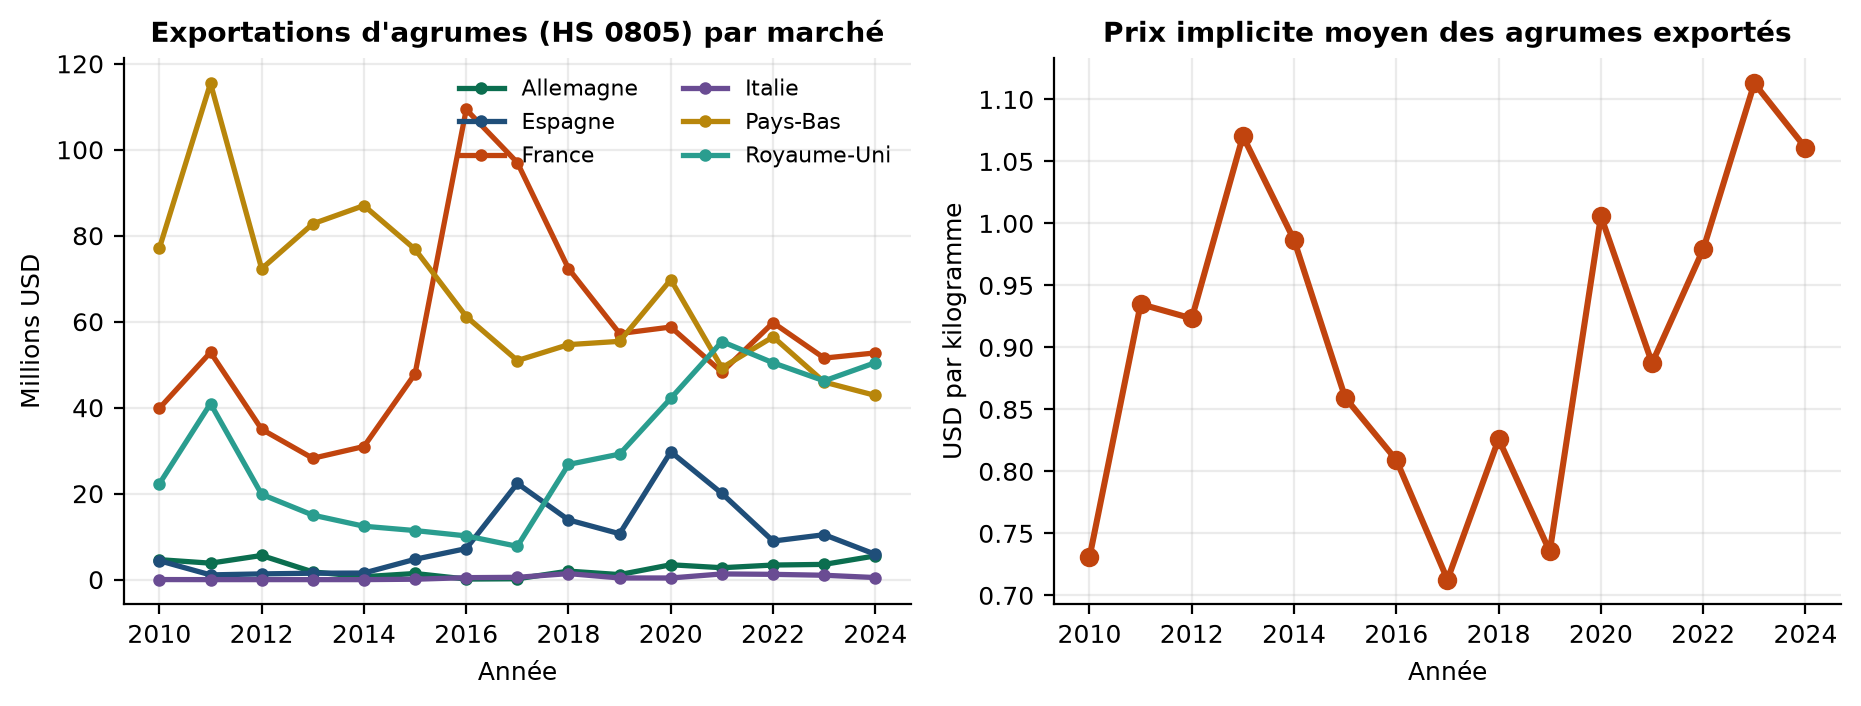
\includegraphics[width=0.82\textwidth]{../figures/fig04_agrumes.png}
  \end{center}
  \vspace{-0.4em}
  \begin{itemize}
    \item Prix implicite : \textbf{0,73 $\to$ 1,06 USD/kg} (+45 \% entre 2010 et 2024).
    \item La valeur des agrumes progresse, mais \textbf{le volume ne suit pas} :
          l'essentiel de la croissance est un effet \textbf{prix}.
    \item Conséquence : un pilotage en valeur seule \textbf{surévalue} la
          performance commerciale.
  \end{itemize}
  \src{Prix implicite = valeur exportée / poids net déclarés à Comtrade.}
\end{frame}

% ---------------------------------------------------------------- 8
\begin{frame}{La concentration reste le premier risque}
  \begin{center}
    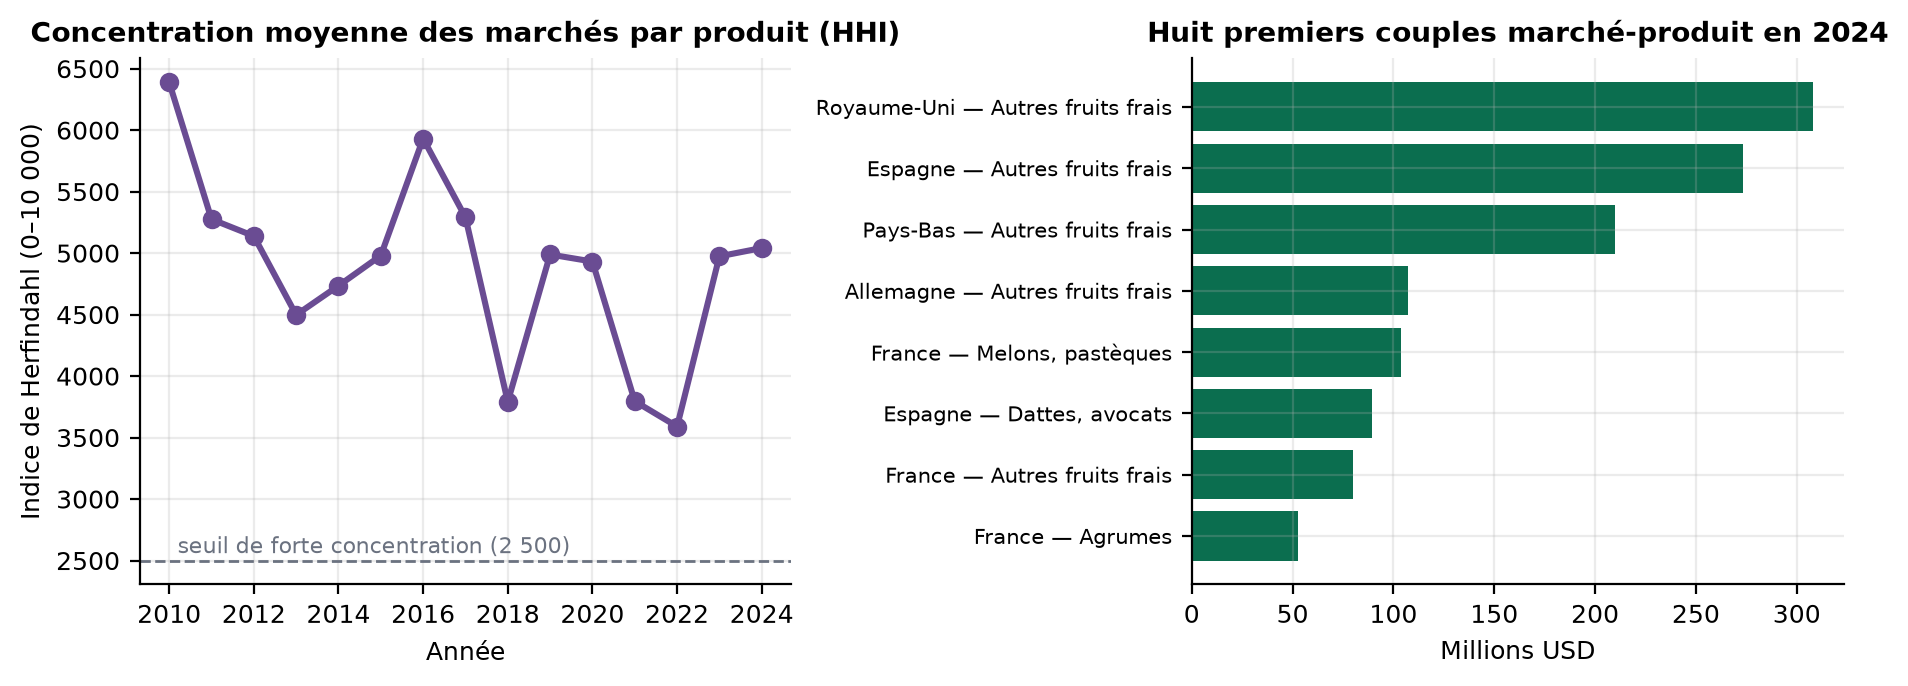
\includegraphics[width=0.80\textwidth]{../figures/fig05_concentration.png}
  \end{center}
  \vspace{-0.5em}
  \begin{columns}[T,onlytextwidth]
    \begin{column}{0.48\textwidth}
      \begin{itemize}
        \item Indice de Herfindahl : \textbf{6\,388 $\to$ 5\,042}
              (2010 $\to$ 2024).
        \item Toujours au-dessus du seuil de \textbf{forte concentration}
              (2\,500).
      \end{itemize}
    \end{column}
    \begin{column}{0.48\textwidth}
      \begin{itemize}
        \item Les \textbf{3 premiers couples} (RU--0810, ES--0810, NL--0810)
              pèsent \textbf{49,2 \%}.
        \item La diversification annoncée dans les plans sectoriels
              \textbf{ne se lit pas encore}.
      \end{itemize}
    \end{column}
  \end{columns}
\end{frame}

% ---------------------------------------------------------------- 9
\begin{frame}{Un protocole sans fuite temporelle}
  \begin{center}
    \begin{tabular}{@{}p{0.25\textwidth}p{0.24\textwidth}p{0.42\textwidth}@{}}
      \toprule
      \textbf{Bloc} & \textbf{Période} & \textbf{Usage} \\
      \midrule
      Entraînement & $t \leq 2019$ & Cibles 2011--2020 \\
      Validation glissante & 6 fenêtres 2016$\to$2017 \ldots 2021$\to$2022
        & Choix des hyperparamètres \\
      Test final & $t = 2022$--$2023$ & Cibles 2023--2024 (108 obs.), utilisé une seule fois \\
      \bottomrule
    \end{tabular}
  \end{center}

  \vspace{0.7em}
  \begin{columns}[T,onlytextwidth]
    \begin{column}{0.31\textwidth}
      \begin{block}{Cible}
        \small $y_{t+1}$ en $\log(1+y)$, reconstruite par \texttt{expm1}.
      \end{block}
    \end{column}
    \begin{column}{0.31\textwidth}
      \begin{block}{Variables}
        \small Retards $t$ à $t-3$, moyennes passées, part de marché,
        croissance mondiale : \textbf{tout est connu fin $t$}.
      \end{block}
    \end{column}
    \begin{column}{0.31\textwidth}
      \begin{block}{Prétraitement}
        \small Indicateurs marché/produit + standardisation, dans un
        \texttt{Pipeline} \textbf{réajusté à chaque fenêtre}.
      \end{block}
    \end{column}
  \end{columns}

  \vfill
  \small\color{vertfonce}\textbf{Aucune statistique calculée sur le test ne contamine l'entraînement.}
\end{frame}

% ---------------------------------------------------------------- 10
\begin{frame}{Quatre modèles, une même règle du jeu}
  \begin{columns}[T,onlytextwidth]
    \begin{column}{0.55\textwidth}
      \textbf{Modèles comparés}
      \begin{itemize}
        \item \textbf{Persistance} : $\hat y_{t+1} = y_t$ (référence).
        \item \textbf{Ridge} : régularisation forte ($\alpha = 100$).
        \item \textbf{Forêt aléatoire} : 600 arbres, feuille $\geq 15$,
              \texttt{max\_features} $= 0{,}5$.
        \item \textbf{Gradient boosting} : perte absolue, taux 0,02,
              200 itérations.
      \end{itemize}
      \vspace{0.3em}
      \small Métriques : MAE, RMSE, \textbf{WAPE} et \textbf{MASE} rapporté
      à la persistance.
    \end{column}
    \begin{column}{0.43\textwidth}
      \textbf{Validation glissante (WAPE moyen)}
      \begin{tabular}{lr}
        \toprule
        Modèle & WAPE \\
        \midrule
        Persistance & \textbf{0,297} \\
        Forêt aléatoire & 0,314 \\
        Gradient boosting & 0,314 \\
        Ridge & 0,381 \\
        \bottomrule
      \end{tabular}
      \vspace{0.5em}

      \small La persistance gagne la validation : les arbres ne démontrent
      pas encore leur supériorité.
    \end{column}
  \end{columns}

  \vfill
  \begin{center}
    \parbox{0.78\textwidth}{\centering\small\color{vertfonce}\textbf{Un
    benchmark volontairement simple : si un modèle complexe ne bat pas
    $y_t = y_{t-1}$, il n'apporte pas de valeur.}}
  \end{center}
\end{frame}

% ---------------------------------------------------------------- 11
\begin{frame}{Test final : un gain réel mais fragile}
  \begin{columns}[T,onlytextwidth]
    \begin{column}{0.55\textwidth}
      \begin{tabular}{lrrr}
        \toprule
        Modèle & MAE & RMSE & WAPE \\
        \midrule
        Persistance & 7,11 & 17,19 & 0,262 \\
        Ridge & 10,71 & 29,53 & 0,395 \\
        \textbf{Forêt aléatoire} & \textbf{6,90} & \textbf{16,37} & \textbf{0,255} \\
        Gradient boosting & 8,00 & 18,06 & 0,295 \\
        \bottomrule
      \end{tabular}
      \vspace{0.5em}

      \small Erreurs en M USD, test 2023--2024 (108 observations).
    \end{column}
    \begin{column}{0.43\textwidth}
      \begin{block}{Lecture}
        \small La forêt aléatoire réduit l'erreur de \textbf{2,9 \%}
        (MASE 0,971), mais son WAPE de validation (0,314) reste
        \textbf{au-dessus} de la persistance (0,297).
      \end{block}
      \vspace{0.5em}
      \small\textbf{Le gain dépend donc de la fenêtre :} il n'est pas
      structurel.
    \end{column}
  \end{columns}

  \vfill
  \begin{center}
    \small\color{vertfonce}Un seul test ne suffit pas à conclure : c'est la
    validation glissante qui tranche.
  \end{center}
\end{frame}

% ---------------------------------------------------------------- 12
\begin{frame}{Prévisions contre réalisations}
  \begin{center}
    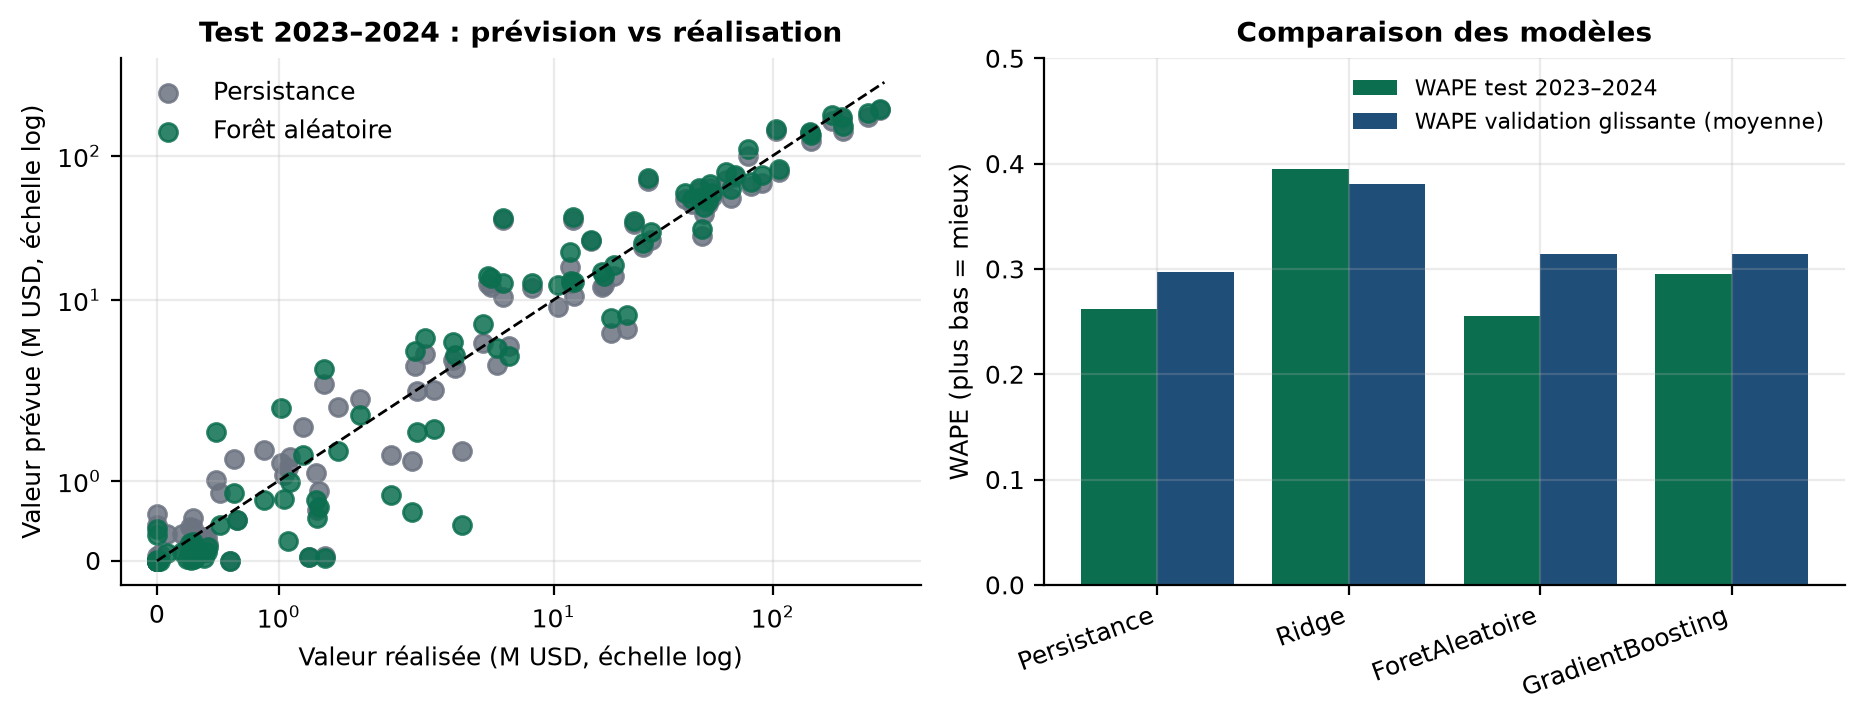
\includegraphics[width=0.90\textwidth]{../figures/fig06_comparaison_modeles.png}
  \end{center}
  \vspace{-0.4em}
  \begin{columns}[T,onlytextwidth]
    \begin{column}{0.48\textwidth}
      \small À gauche : chaque point est un couple (marché, produit) du test.
      Les gros flux suivent la diagonale ; les petits sont dispersés.
    \end{column}
    \begin{column}{0.48\textwidth}
      \small À droite : la forêt aléatoire est devant sur le test, derrière
      en validation. La hiérarchie n'est pas stable.
    \end{column}
  \end{columns}
\end{frame}

% ---------------------------------------------------------------- 13
\begin{frame}{Où le modèle gagne, où il perd}
  \begin{columns}[T,onlytextwidth]
    \begin{column}{0.48\textwidth}
      \textbf{WAPE par marché (test)}
      \begin{tabular}{lrr}
        \toprule
        Marché & Persist. & Forêt \\
        \midrule
        France & \textbf{0,182} & 0,199 \\
        Royaume-Uni & 0,244 & \textbf{0,230} \\
        Espagne & 0,267 & \textbf{0,233} \\
        Pays-Bas & 0,273 & \textbf{0,238} \\
        Allemagne & \textbf{0,426} & 0,478 \\
        Italie & \textbf{0,650} & 0,935 \\
        \bottomrule
      \end{tabular}
      \vspace{0.4em}

      \small Le gain se concentre sur les \textbf{gros flux} (ES, NL, RU) ;
      la persistance reste meilleure sur les marchés stables ou petits.
    \end{column}
    \begin{column}{0.48\textwidth}
      \textbf{Ce qui porte la prévision}\\
      \small Importance par permutation (forêt, test) :
      \begin{itemize}
        \item valeur retardée $y_t$ : \textbf{0,054} ;
        \item moyenne des 3 derniers logarithmes : \textbf{0,040} ;
        \item part de marché : \textbf{0,031} ;
        \item contexte mondial (croissance, total) : \textbf{$\approx 0$}.
      \end{itemize}
      \vspace{0.3em}
      \small Autrement dit, \textbf{le passé du couple} contient l'essentiel
      de ce que le modèle peut apprendre.
    \end{column}
  \end{columns}
\end{frame}

% ---------------------------------------------------------------- 14
\begin{frame}{Robustesse et projection 2025}
  \begin{columns}[T,onlytextwidth]
    \begin{column}{0.50\textwidth}
      \textbf{Tests de sensibilité (WAPE)}
      \begin{tabular}{lrr}
        \toprule
        Scénario & Persist. & Forêt \\
        \midrule
        Principal & 0,262 & 0,255 \\
        S1 sans zéros imputés & -- & 0,253 \\
        S2 test 2020--2024 & 0,297 & 0,308 \\
        S3 sans produit 0810 & 0,298 & 0,288 \\
        \bottomrule
      \end{tabular}
      \vspace{0.4em}

      \small L'ordre des modèles \textbf{change selon le scénario} : le gain
      de la forêt n'est pas structurel.
    \end{column}
    \begin{column}{0.46\textwidth}
      \begin{block}{Projection 2025 (scénario de cadrage)}
        \small Total : \textbf{1\,771,3 \MUSD} [1\,607,8 ; 1\,977,4],
        soit \textbf{+10,2 \%}.\\[0.3em]
        Espagne 471,5 ; Royaume-Uni 414,0 ; Pays-Bas 362,8 ; France 345,2 ;
        Allemagne 163,1 ; Italie 14,6.
      \end{block}
      \vspace{0.3em}
      \scriptsize Intervalle empirique à 80 \%, construit sur les erreurs
      relatives du backtest roulant 2014--2024. Ce n'est pas un engagement
      contractuel.
    \end{column}
  \end{columns}
\end{frame}

% ---------------------------------------------------------------- 15
\begin{frame}{Conclusion : trois messages}
  \begin{enumerate}
    \item \textbf{La valeur ajoutée n'est pas la prévision ponctuelle, mais la
          lecture des écarts.} Les couples se comportent comme des marchés
          aléatoires à fréquence annuelle ; le modèle sert à \emph{signaler}
          un changement, pas à le prédire au dixième.
    \item \textbf{La croissance est largement une croissance de prix.}
          Le prix implicite des agrumes progresse de 45 \% ; un pilotage en
          valeur seule surévalue la performance commerciale.
    \item \textbf{La concentration reste le premier risque.}
          Trois couples = 49,2 \% de la valeur. La diversification
          (Allemagne, Royaume-Uni, UE) est un levier plus sûr qu'une
          optimisation de modèle.
  \end{enumerate}

  \vspace{0.3em}
  \begin{block}{Limites et perspectives}
    \small 15 points annuels, montants nominaux, pas de saisonnalité, hub
    néerlandais, zéros imputés. Priorités : passage au \textbf{mensuel},
    variables exogènes (prix, taux de change, logistique), prévision
    \textbf{par intervalle}.
  \end{block}

  \vfill
  \begin{center}
    \Large\color{vertfonce}\textbf{Merci de votre attention. Questions ?}
  \end{center}
\end{frame}

\end{document}
